\documentclass[12pt]{article}

% Packages
\usepackage[a4paper,left=2.5cm,right=2.5cm,top=2.5cm,bottom=2.5cm,footskip=1cm]{geometry}
\usepackage{xcolor} \usepackage[explicit]{titlesec}
\usepackage[colorlinks=false]{hyperref} \usepackage{graphicx}
\usepackage{caption}
\usepackage[parfill]{parskip}
\usepackage[ngerman]{babel}
\usepackage{microtype}
\usepackage{csquotes}
\usepackage{color}
\usepackage{csquotes}
\usepackage{listings}

\lstset{
    basicstyle=\ttfamily\scriptsize,
    % basicstyle=\ttfamily\small,
    frame=lines,
    framesep=2pt,
    xleftmargin=0pt,
    xrightmargin=0pt,
    numberstyle=\tiny,
    numbers=left,
}


% Settings
\hypersetup{pdfborder=0 0 0} \definecolor{FomBlue}{HTML}{00998A}
\linespread{1.20}

% Title page

\title{
    
\includegraphics[width=5cm]{images/logo.png}
    \\
    \vspace{1cm}
    \textbf{Big-Data-Analyseprojekt}\\ \bigskip \large Analyse der Auswirkungen
    verschiedener Pruning-Methoden an \emph{Large Language Models}
}
\author{Kai Daniel Herbst und Sebastian Viet}
\date{Oktober 2024 - März 2025}


% Document
\begin{document}
\begin{sloppypar}
	\maketitle
	\thispagestyle{empty}

	\newpage
	\setcounter{page}{1}
	\pagenumbering{Roman}

	\renewcommand{\contentsname}{Inhaltsverzeichnis}
	\tableofcontents

	\newpage
	\setcounter{page}{1}
	\pagenumbering{arabic}

	Ziel: 3600 Wörter

	\section{Einleitung}

\subsection{Forschungsfragen}

Die vorliegende Projektarbeit setzt sich mit insgesamt vier Forschungsfragen
auseinander, die im Verlauf der Arbeit untersucht und beantwortet werden sollen.
Die erste Forschungsfrage beschäftigt sich mit dem aktuellen Stand der Forschung
im Bereich des Prunings von Large Language Models (LLMs). Dabei wird analysiert,
welche Methoden derzeit für das Pruning angewendet werden, welche Unterschiede
zwischen diesen bestehen und welche Vor- und Nachteile die jeweiligen Ansätze
mit sich bringen. Das Ziel dieser Untersuchung ist es, einen Überblick über den
aktuellen Stand der Forschung in diesem Bereich zu geben und die relevantesten
Methoden zu beschreiben.

Ein weiterer Aspekt dieser Arbeit ist die Analyse der verschiedenen Frameworks,
die Pruning-Methoden für LLMs unterstützen. Hierbei soll untersucht werden,
welche dieser Frameworks welche Methoden implementieren und wie sie in der
Praxis angewendet werden können. Basierend auf dieser Analyse wird eine
geeignete Auswahl getroffen und eines dieser Framework für die praktische
Umsetzung festgelegt.

Neben der theoretischen Auseinandersetzung mit dem Thema wird zudem ein eigener
praktischer Versuch durchgeführt. Hierzu wird ein geeignetes Basismodell
ausgewählt, das anschließend in verschiedenen Stufen geprunt wird. Die
Auswirkungen dieses Prunings werden untersucht und dokumentiert. Im Rahmen
dieser Analyse werden standardisierte Benchmarks erstellt, um die geprunten
Modelle zu bewerten. Dabei wird nicht nur die Performance hinsichtlich der
Ergebnisse in den Tests betrachtet, sondern auch der Einfluss des Prunings auf
den Speicherverbrauch und die benötigte Rechenzeit. Ziel ist es, Erkenntnisse
darüber zu gewinnen, wie sich das Pruning auf verschiedene Aspekte der Modelle
auswirkt.

Zusammenfassend ergeben sich daraus die folgenden Forschungsfragen:

\begin{enumerate}
	\item Wie ist der aktuelle Stand der Forschung im Bereich des
	      Prunings von Large Language Models, und welche Methoden werden derzeit
	      eingesetzt?
	\item Welche Frameworks bieten Unterstützung für das Pruning von
	      LLMs, und wie lassen sich diese in der Praxis anwenden?
	\item Welche
	      Auswirkungen hat das Pruning eines Modells auf dessen Leistungsfähigkeit in
	      Bezug auf standardisierte Benchmarks und Aufgaben?
	\item Inwiefern
	      beeinflusst das Pruning eines Modells dessen Speicherverbrauch sowie die
	      benötigte Rechenzeit?
\end{enumerate}

	\section{Theoretische Grundlagen}

\subsection{Übersicht über Large Language Models}

Large Language Models (LLMs) stellen ein bedeutendes Forschungsfeld innerhalb
der künstlichen Intelligenz (KI) dar. Sie basieren auf komplexen neuronalen
Netzwerken, die auf die Generierung und Verarbeitung natürlicher Sprache
spezialisiert sind, und gehören zur Klasse der Foundation Models. Bekannte
Beispiele hierfür sind ChatGPT (OpenAI), Llama (Meta), Bard (Google) oder
DeepSeek (Lian Wenfeng). Insbesondere Unternehmen zeigen großes Interesse an
der Nutzung dieser Modelle, da sie ein erhebliches Potenzial zur Steigerung
der Produktivität bieten. Der aktuelle Trend zeigt, dass LLMs zunehmend in
bestehende Software integriert oder bei Neuentwicklungen unmittelbar
berücksichtigt werden \autocites[Vgl.][S. 1-2,5]{lu2024taxonomy}[S. 1-2]{minaee2024survey}

Das Training von LLMs erfolgt auf Basis des Generative Pretrained
TransformerAnsatzes (GPT). Durch Mechanismen wie Gewichtung (Attention) und
SelfSupervised Learning wird die Vorhersage des nächsten Tokens ermöglicht.
Die zugrunde liegenden Trainingsdatensätze umfassen oft mehrere Petabytes, was
den Modellen erlaubt, trotz breiter Themenvielfalt komplexe Zusammenhänge zu
erkennen. Darüber hinaus entwickeln LLMs emergente Fähigkeiten wie In-Context
Learning oder MultiStep Reasoning \autocites[Vgl.][S. 6-10]{lu2024taxonomy}{lu2024taxonomy}[S. 1-2]{minaee2024survey}[S. 1-2]{naveed2024overview}.

Aufgrund der hohen Anzahl an Parametern und der großen Datenmengen erfordern
sowohl das Training als auch der Betrieb von LLMs erhebliche Rechenressourcen.
Zur Reduzierung dieser Anforderungen werden für spezifische Anwendungsbereiche
Small Language Models (SLMs) entwickelt. Diese Modelle sind weniger
ressourcenintensiv und neigen zu geringeren Halluzinationen, sofern die
Gesprächsthematik mit ihrer trainierten Spezialisierung übereinstimmt. Ein
weiterer vielversprechender Ansatz besteht darin, Halluzinationen zunächst
durch ein SLM zu identifizieren und anschließend mithilfe eines nachgelagerten
LLMs sowie dessen Constraint-Based Reasoning-Funktion hinsichtlich Konsistenz
und Logik zu verbessern. Huang, Yu, Ma et al. betonen, dass die Bereitstellung
verfeinerter Halluzinationskategorien es LLMs ermöglicht, Halluzinationen
zuverlässiger zu erkennen \autocites[Vlg.][]{kelbert2023llm}{huang2024hallucination}[S. 6-14]{hu2024slm}

\subsection{Effizienzoptimierung mittels Pruning}


Bei Pruning handelt es sich um eine Methode zur Reduktion der Komplexität und
Größe bei Modellen. Sie findet Anwendung im Bereich der Entscheidungsbäume und
neuronalen Netzen. Die Effizienzsteigerung wird durch die Entfernung
irrelevanter Teile erzielt. Pruning kann in drei Unterkategorien unterteilt
werden: strukturelles, unstrukturelles und adaptives Pruning. Diese werden
folgend weiter vorgestellt. Der Schwerpunkt wird auf strukturelles Pruning
gelegt, da dieses auch später im Praxisteil Anwendung findet.

Das Kapitel wird durch die Vorstellung einer weiteren Unterscheidungsvariante
aus einer Metastudie von Vadera und Ameen abgerundet.

\subsubsection{Strukturelles Pruning}

Beim strukturellen Pruning werden ganze Teileinheiten wie Filter oder Kanäle
aus dem neuronalen Netz entfernt. Die Modelle werden kompakter und dadurch auch
auf Standardhardware ausführbar. Ebenso die gute Kompatibilität zu
Standardbibliotheken aus dem Deep Learning-Segment und die Möglichkeit das
Pruning mit weiteren Kompressionsverfahren zu kombinieren, machen den Ansatz
attraktiv. Beides wirkt sich positiv auf die entstehenden Kosten aus.
\autocites[Vgl.][S. 1]{he2023structured}[S. 1-2]{vadera2022methods}

Die Ausgangslage ist ein bereits trainiertes Netz. Die Herausforderung beim
Pruning ist die Identifizierung der Teileinheiten, die ohne Verlust an
Modellgenauigkeit löschbar sind. Zum einen kann die Selektion gewichtsabhängig
erfolgen. Hierfür werden z.B. anhand des geometrischen Medians redundante
Filter identifiziert. Alternativ ist eine Betrachtung der L1-Norm (Summe aller
Absolutwerte eines Vektors) und L2-Norm (Quadratwurzel der Summe der Quadrate
der Einträge eines Vektors) möglich. Filter mit kleinen Summen werden entfernt.
Hierbei spricht man von magnitudenbasierten Metriken. Neben der Betrachtung
der Gewichte kann auch die Aktivierung als Kriterium genutzt werden. Der
Rekonstruktionsfehler, der durchschnittliche Rang oder die Anzahl an Nullen
auf den Aktivierungskarten werden als Kriterien für die Eliminierung genutzt.
Über eine Kreuzkorrelation kann zudem die Unabhängigkeit eines Kanals bestimmt
werden. Mit der Taylor-Expansion kann der entstehende Verlustwert nach
Entfernung eines Filters möglichst annähernd ermittelt werden. He und Xian
ordnen die Taylor-Expansion der Unterkategorie optimierungsbasierten Methoden
zu, während Vadera und Ameen den Ansatz zur Gruppe der Sensitivity Analysis
zählen. Unabhängig von der gewählten Methode ist es wichtig nach der Entfernung
von Strukturen ein Finetuning vorzunehmen. Dieses dient dazu die Leistung zu
optimieren und soll auftretende Genauigkeitsverluste auszugleichen. \autocites[Vgl.][S. 1-5]{he2023structured}[S. 1-5]{vadera2022methods}

\subsubsection{Unstrukturelles Pruning}

Während beim strukturellen Pruning ganze Neuronen, Kanäle oder Filter entfernt
werden, wird beim unstrukturellen Pruning jede Gewichtsverbindung analysiert
und bewertet. Die Zielsetzung besteht erneut darin, überflüssige Informationen
zu entfernen. Die Reduktion führt jedoch zu einer reduzierten Gewichtsmatrix
mit unregelmäßigen Mustern. Die Umsetzung erfolgt meist über
Maskierungstechniken. Diese deaktivieren durch binäre Masken unwichtige
Gewichte. \autocite[Vlg.][S. 3]{cheng2024survey}

Da klassische GPUs auf dichte Matrizen optimiert sind, erfordert der Einsatz
spezielle Hard- und Software. Es handelt sich somit um eine kostenintensivere
Variante als das strukturierte Pruning. Die Bewertung jedes einzelnen Gewichts
lässt zwar eine sehr feine Kontrolle über die Einsparung zu, jedoch kann das
fehlerhafte Entfernen einer einzelnen kritischen Verbindung bereits zu
Informationsverlust führen. Unter sorgfältiger Berücksichtigung dieser Gefahr
kann jedoch ein hoher Kompressionsgrad erzielt werden. So zeigen Zhu und Gupta
mittels Pruning verschiedener neuronaler Architekturen, dass eine Kompression
ohne Leistungsbeeinträchtigung um bis 90\% möglich ist.\autocites[Vgl.][S.3]{cheng2024survey}[S. 6-8]{zhu2022prune}

\subsubsection{Adaptive Pruning Verfahren}

Im Gegensatz zu traditionellen Pruning-Verfahren, bei denen die Kriterien im
Voraus festgelegt werden, erfolgt das adaptive Pruning dynamisch während des
Trainings. Das Verfahren passt sich dynamisch an Änderungen wie Gewichte,
Gradienten oder Aktivierungen an und maximiert so die Effizienz. Manuelle
Anpassungen werden auf ein Minimum beschränkt. Auch die komplexe Ermittlung
von Parametern, die universell für das vollständige Modell gelten könnten,
entfällt. Wie beim unstrukturierten Pruning muss die Hardware jedoch sparse
Matrizen verarbeiten können. Im Gegenzug ist adaptives Pruning sehr flexibel
und somit ideal für ressourcenbegrenzte Geräte. Beispielsbereiche sind das
autonome Fahren sowie moderne Smartphones und Tablets mit dedizierten KI-Chips.

Prominente Beispiele sind das Layer-Adaptive-Pruning oder das Adaptive
Channel-Pruning. Ersteres leitet die unterschiedlichen Pruning-Raten je Schicht
aus der Sensitivität ab. Letzteres arbeitet mit der Entfernung von Kanälen in
CNNs. \autocites[Vgl.][S. 295-296]{sakai2022structured}[S. 1-2]{wang2025adapt}


\subsubsection{Weitere Möglichkeiten der Kategorisierung von Pruning}

In einer Metastudie haben Vadera und Ameen über 150 Paper zu Pruning
untersucht. Hierbei gruppierten sie die Veröffentlichungen nicht nach
strukturiert, unstrukturiert und adaptiv, sondern nach dem verwendeten
(mathematischen) Ansatz. Es konnten acht Kategorien gebildet werden, die kurz
benannt und vorgestellt werden:\autocite[Vgl.][S. 2]{vadera2022methods}

\begin{itemize}
	\item \textbf{Magnitude-based Pruning Methods:} Relevanz von Gewichten und Neuronen wird über lokale Maße wie z. B. die Magnitude bestimmt.
	\item \textbf{Similarity and Clustering Methods:} Identifizierung und Entfernung redundanter oder sehr ähnlicher Gewichte.
	\item \textbf{Sensitivity Analysis Methods:} Entfernung der Gewichte, die geringen Einfluss auf das Endergebnis haben.
	\item \textbf{Knowledge Distillation Methods:} Ableitung eines neuen Modells („Student“) aus dem Ursprungsmodell („Teacher“).
	\item \textbf{Low-Rank Methods:} Zerlegung der Gewichtsmatrix in ein Produkt aus zwei kleineren Matrizen.
	\item \textbf{Quantization Methods:} Verwendung von Hashing, niedriger Präzision oder binärer Darstellung, um die Berechnungsaufwände zu reduzieren.
	\item \textbf{Architectural Design Methods:} Nutzung von Such- und Reinforcement-Learning zur Erstellung neuronaler Netzwerkarchitekturen.
	\item \textbf{Hybrid Methods:} Kombination mehrerer Ansätze zur Steigerung der Kompressionseffekte.
\end{itemize}

Erwähnenswert ist zudem, dass diese acht Kategorien teilweise noch feiner
unterteilt werden konnten. Abbildung 1 zeigt eine Auswahl aus den ersten drei
Kategorien der Metastudie.

\begin{figure}[H]
	\centering
	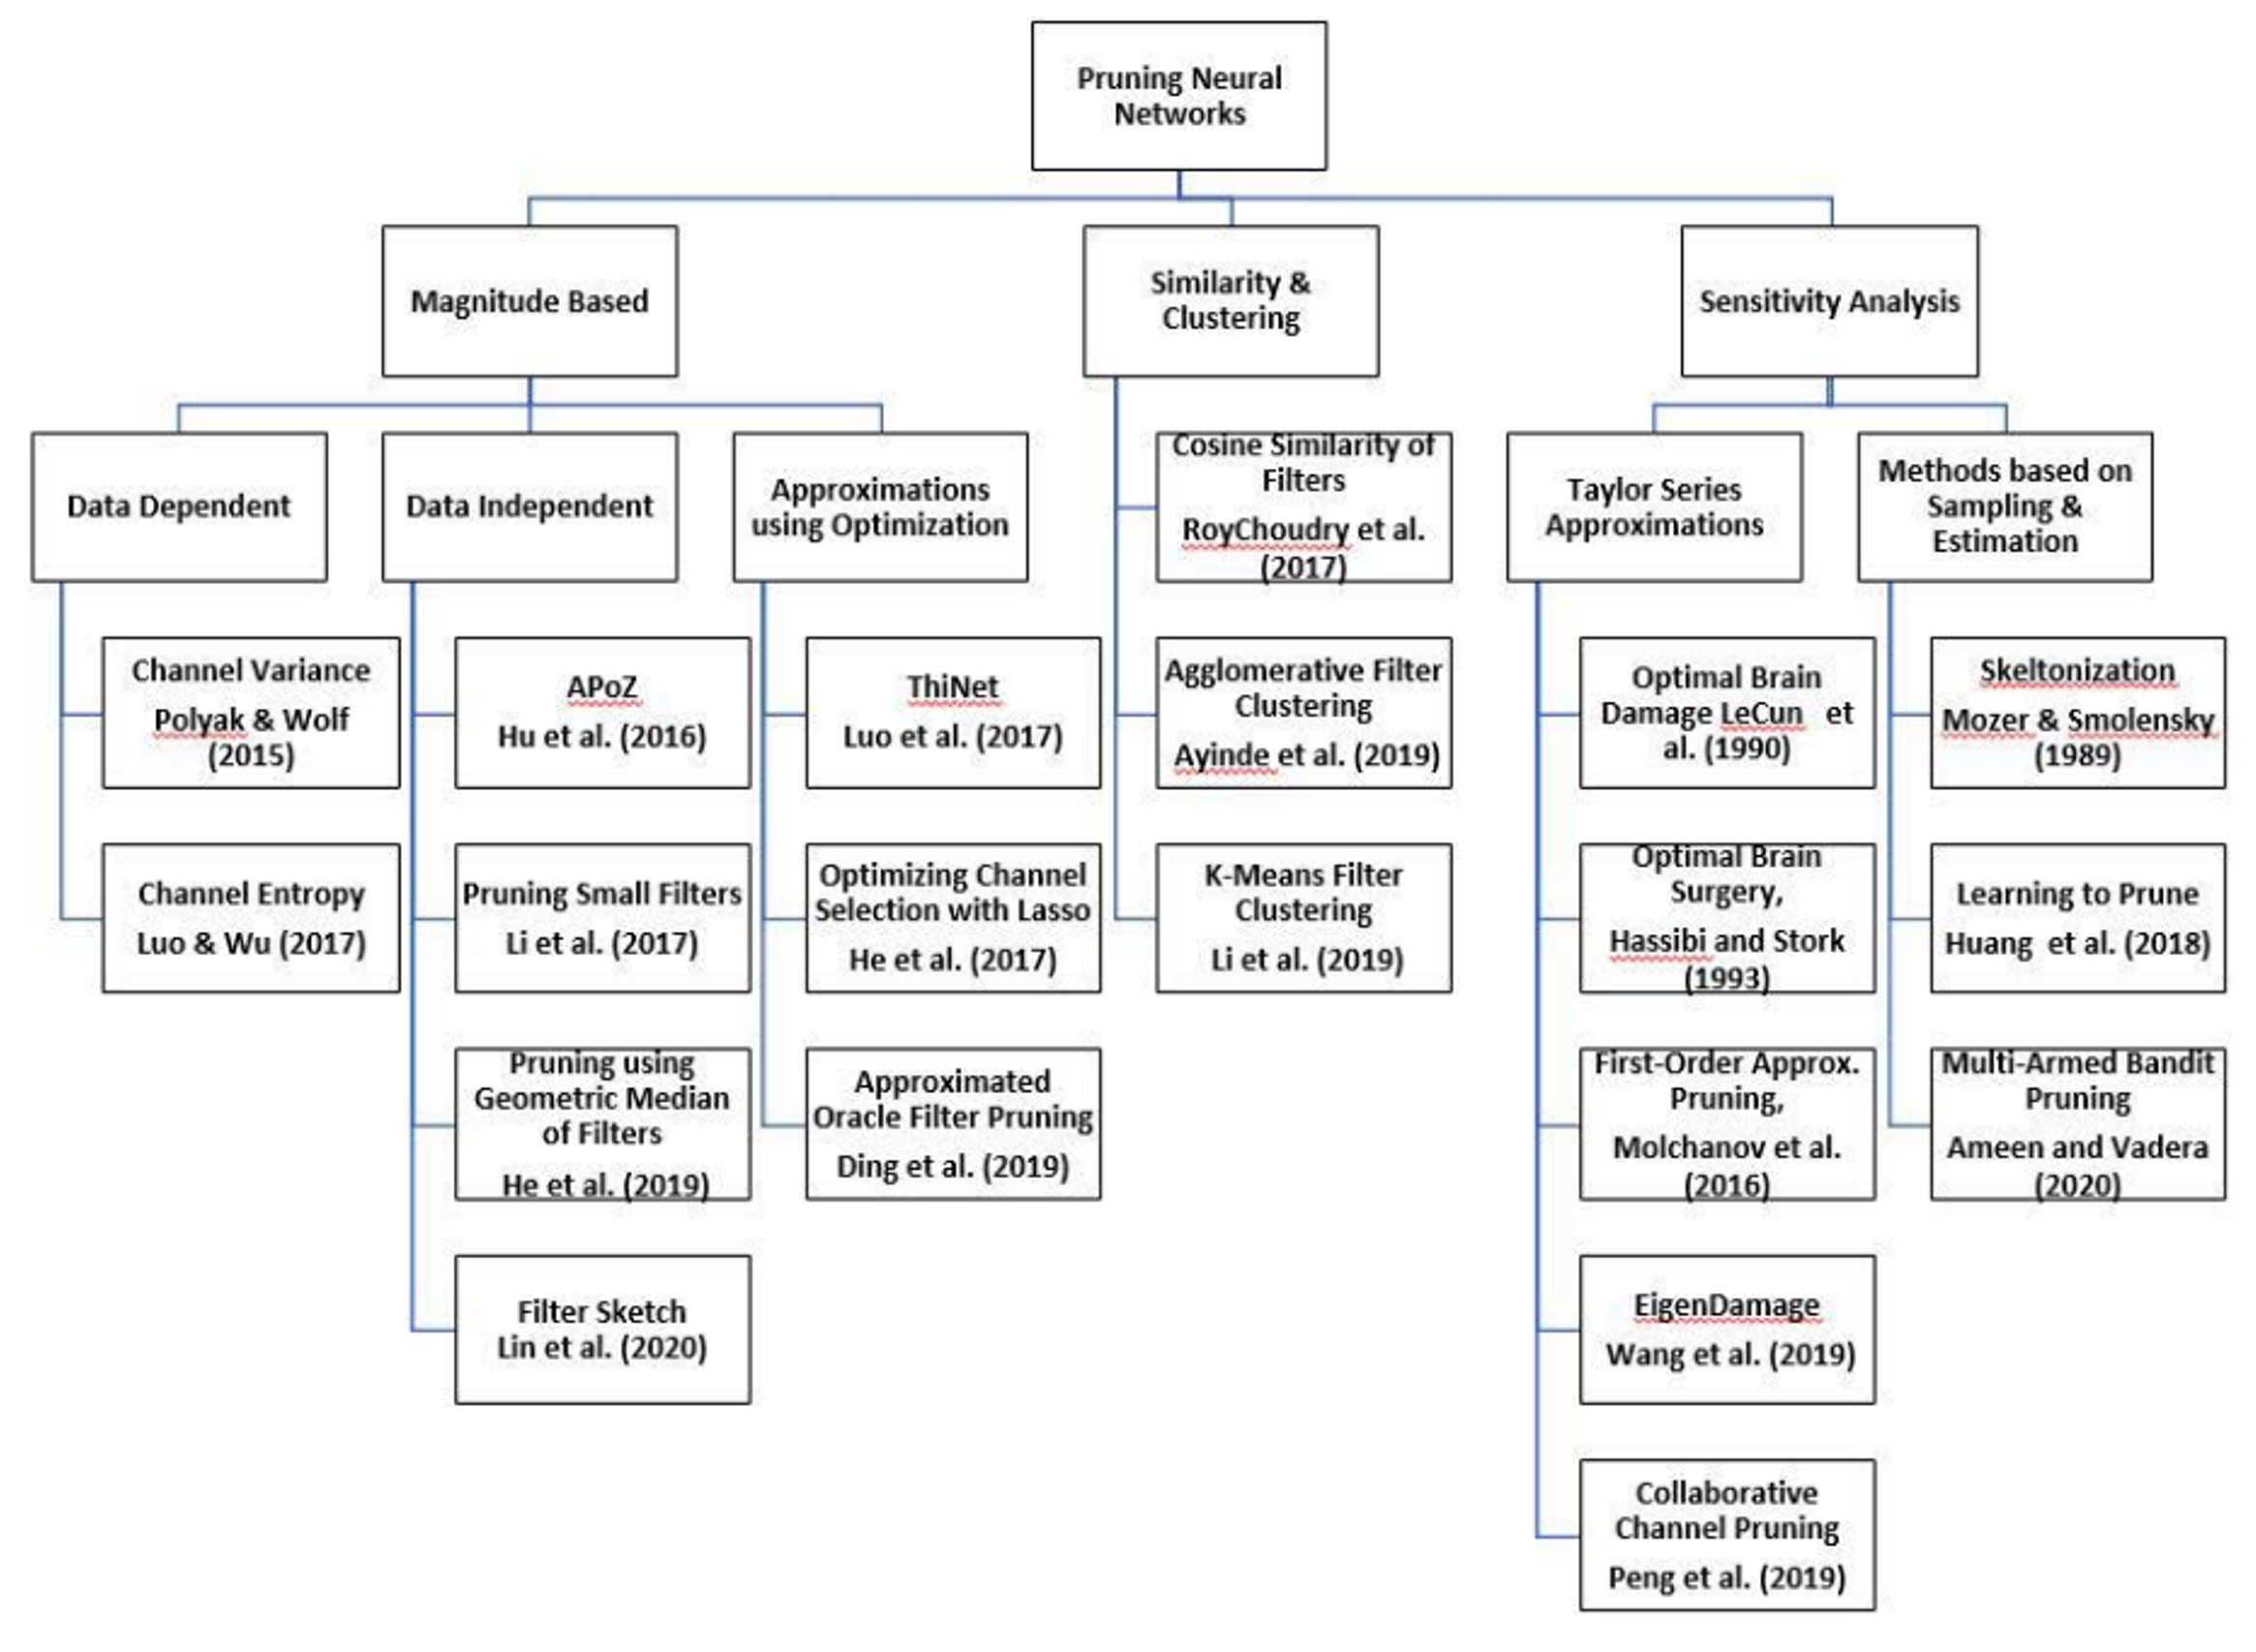
\includegraphics[width=0.9\textwidth]{images/pruning.png}
	\caption{Aufteilung nach Vadera und Ameen\\Quelle: \cite{vadera2022methods}}
	\label{fig:vadera}
\end{figure}


\newpage
\subsection{Bewertungskriterien}

Um die Effizienz der unterschiedlichen Pruning-Ansätze zu ermitteln, ist das
Heranziehen des Random-Pruning als Vergleichsmethode beliebt. Li, Adamczewski
et al. unterscheiden dabei in drei verschiedene Wege, wie das Random-Pruning
umgesetzt werden kann:

\begin{itemize}
	\item \textbf{Vollständig zufällig:} Das Pruning findet zufällig und ohne weitere Vorgaben statt.
	\item \textbf{Eingeschränkt zufällig:} Das Pruning-Verhältnis wird je Schicht vorgegeben. Innerhalb der Schicht erfolgt das Pruning jedoch weiterhin zufällig.
    \item \textbf{Zufällige Kanalanzahlauswahl:} Das Pruning-Verhältnis wird je Schicht zufällig ausgewählt.\autocite[Vgl.][]{li2022random}
\end{itemize}

Sowohl He und Xiao als auch Li, Adamczewski et al. konstatieren in ihren
Untersuchungen ein überraschend gutes Abschneiden des Random-Prunings im
Vergleich zu weiterentwickelten Methoden.\autocites[Vgl.][]{he2023structured}{li2022random}

Relevanter ist jedoch die Frage, inwieweit das Sprachmodell nach dem Pruning
noch „funktionsfähig“ ist. Hierunter wird die Fähigkeit verstanden Eingaben in
das Modell auf plausible Weise zu beantworten. Zur Untersuchung kommen extra
auf diese Fragestellung zugeschnittene Benchmarks zum Einsatz. Diese enthalten
Testfragen, welche an das Sprachmodell gestellt werden, sowie zugehörige
Lösungen, die mit den Antworten des LLMs in Anschluss abgeglichen werden. Bei
der Auswahl des Benchmark-Modells ist auf dessen Prüfziele zu achten. So
unterscheiden sich die Modelle im Schwierigkeitsgrad und in der Breite der
Themenabfrage. Die im Projekt eingesetzten Benchmark-Modelle werden im
Folgenden kurz vorgestellt.


\begin{itemize}
    \item \textbf{BoolQ (Boolean Questions):} Der Datensatz enthält 15.942 Ja-/Nein-Fragen. Die Fragen sind realen Kontexten entnommen und nicht generiert worden. Neben der Fragestellung wird dem LLM ein Begleittext mitgegeben, welcher die Antwort auf die Frage bzw. Hilfestellungen enthält. Hierbei wird jedoch oft auf komplexere Schlussfolgerungen durch die KI gesetzt. Als einfaches Beispiel zum Verständnis sei folgender Begleittext gegeben: Spanien hat die Fußball-EM 2024 gewonnen. Die zugehörige Frage lautet: Hat Harry Kane die EM 2024 gewonnen? Die KI muss nun trotz ihres reduzierten neuronalen Netzes erkennen, dass Harry Kane zwar ein Fußballspieler ist, aber als Nationalspieler für England und nicht für Spanien im Finale antrat. Die Antwort muss daher Nein lauten.\autocite[Vgl.][S. 1-2]{clark2019boolq}
    
    \item \textbf{Arc-C (AI2 Reasoning Challenge):} Der Datensatz enthält 7.787 Multiple-Choice-Fragen aus dem naturwissenschaftlichen Bereich auf amerikanischem Grundschulniveau (Klassen 3 bis 9). 2.590 der Fragen werden als besonders herausfordernd klassifiziert. Sie gelten als nicht beantwortbar für abrufbasierte oder Wort-Koexistenz-Algorithmen. Optional wird ein Datensatz mit 14 Millionen wissenschaftlichen Sätzen angeboten, welcher der KI zur Beantwortung der Fragen als Hilfestellung gereicht werden kann.\autocite[Vgl.][S. 1]{clark2019arc}

    \item \textbf{HellaSwag:} Bei HellaSwag handelt es sich um die Weiterentwicklung von Swag. Der Datensatz enthält 39.905 Trainingsdatensätze und 5.021 Datensätze für Test und Validierung. Bei HellaSwag ist für das LLM die Aufgabe, einen gegebenen Satz sinnvoll fortzusetzen. Dem LLM werden dabei 4 mögliche Fortsetzungen angeboten, wovon nur eine richtig ist. Das LLM wird somit auf richtige Schlussfolgerungen basierend auf Alltagswissen getestet. Die drei falschen Antwortmöglichkeiten wurden mittels des Adversarial-Filtering-Verfahrens generiert. Auf Basis von iterativ eingesetzten Diskriminatoren werden die negativen Antworten so gestaltet, dass sie für künstliche Intelligenz schwer zu erkennen sind. Der Mensch hingegen kann die falschen Antworten leicht erkennen.\autocite[Vgl.][S. 1-3]{zellers2019hellaswag}

    \item \textbf{OpenBookQA:} Der Datensatz enthält 5.957 Multiple-Choice-Fragen mit je vier Antwortmöglichkeiten. Wie der Name bereits nahelegt, empfindet der Test Open-Book-Prüfungen nach, bei denen die Prüflinge freien Zugang zu Informationen haben. Das Modell enthält daher zu jeder Frage auch ein \textit{core fact}, welches die unterstützende Wissensquelle imitieren soll. Die Fragen sind so gestaltet, dass eine mehrschrittige Schlussfolgerung unter Einbeziehung von externem Wissen notwendig ist.\autocite[Vgl.][S. 1-2]{mihaylov2018armor}

    \item \textbf{WinoGrande:} Bei WinoGrande handelt es sich um die Weiterentwicklung der Winograd Schema Challenge (WSC). Während das Original nur 273 Aufgaben beinhaltet, setzt die Erweiterung auf 44.000 Problemstellungen. Diese wurden auf Basis von Crowdsourcing erstellt und geprüft. Die Aufgaben sind als \textit{fill-in-the-blank}-Probleme gestellt, wo Pronomen durch ihre richtige Referenz ersetzt werden müssen. Um den Schwierigkeitsgrad anzuheben, wurde zusätzlich AfLite (Adversarial Filtering) angewendet. Dies verhindert die Ausnutzung einfacher Wortassoziationen durch das LLM bei der Beantwortung der Fragen.\autocite[Vgl.][S. 1-3]{sakaguchi2019winogrande}
\end{itemize}

\newpage

	\section{Methodik (Kai Herbst)}\label{methodik}

\subsection{Literaturrecherche}

\subsection{Arbeitsorganisation}

Für die Zusammenarbeit und Organisation der anstehenden Aufgaben und zu
verfassenden Kapitel wurde das Notizenprogramm \emph{Notion} verwendet. Notion
erlaubt das Erstellen kollaborativer Notizbücher, die parallel von mehreren
Personen bearbeitet werden können. Über die Datenbankfunktion lassen sich sowohl
Meilensteinpläne als auch Task-Boards erstellen, die zur Planung der Arbeit
verwendet wurden.

\subsection{Entwicklungsumgebung}

Da sowohl das Pruning von Large Language Models als auch die anschließende
Evaluierung der geprunten Modelle erhebliche Rechenressourcen erfordern, wurde
entschieden, diese Prozesse auf einem leistungsstarken Server in der Cloud
durchzuführen. Insbesondere das Testen der resultierenden Modelle stellt eine
hohe Belastung für die verfügbaren Ressourcen dar und ist auf herkömmlicher
Hardware nicht effizient durchzuführen. Zu diesen Zweck wurden EC2-Instanzen des
Cloud-Providers AWS (Amazon Web Services) aus der \emph{g}-Instanzfamilie
verwendet. Diese Instanzfamilie ist speziell auf rechenintensive Anwendungen
ausgelegt und bietet GPUs (Graphics Processing Units), die für parallele
Berechnungen optimiert sind und den Einsatz von CUDA, dem von \emph{NVIDIA}
entwickelten Toolkit zur Verwendung von GPUs in allgemeinen Rechenaufgaben,
ermöglichen.

Im Detail wurden Instanzen des Typs \emph{gd4n.xlarge} verwendet, die mit 16 GiB
Hauptspeicher, einem leistungsstarken Prozessor der \emph{Intel Xeon Family}
sowie einer \emph{NVIDIA T4 Tensor Core} Grafikeinheit ausgestattet sind. Für
den Start der Instanzen wurde das speziell auf Deep-Learning-Anwendungen
zugeschnittene \emph{Deep Learning OSS Nvidia Driver AMI GPU PyTorch 2.5.1
	(Ubuntu 22.04) 20241208} Ubuntu-Image verwendet. In diesem Image ist das
benötigte Python-Package \emph{PyTorch} bereits vorinstalliert und ist
zusätzlich mit \emph{CUDA} ausgestattet.

\begin{table}[ht!]
	\centering

	\resizebox{\textwidth}{!}{
		\begin{tabular}{|p{3cm}|p{12cm}|}
			\hline
			\multicolumn{2}{|c|}{\textbf{Verwendete EC2-Instanz}}                 \\
			\hline
			Instanz-Typ   & gd4n.xlarge                                           \\
			\hline
			Hauptspeicher & 16GiB                                                 \\
			\hline
			vCPU          & 4                                                     \\
			\hline
			Clock Speed   & 2.5GHz                                                \\
			\hline
			GPU           & nvidia t4 tensor core                                 \\
			\hline
			CPU           & Intel Xeon Family                                     \\
			\hline
			AMI           & Deep Learning OSS Nvidia Driver AMI GPU PyTorch 2.5.1 \\
			\hline
			AMI-ID        & ami-0fa5e5fd27b3e163a                                 \\
			\hline
		\end{tabular}}
	\caption{Attribute der verwendeten Hardware}
\end{table}

Nachdem über SSH (Secure Shell) mit der jeweiligen Instanz verbunde wurde,
wurde zunächst die vorinstallierte PyTorch-Umgebung gestartet und
anschließenden das Repository des verwendeten Frameworks geklont.

\vspace{1em}
\begin{lstlisting}
$ source activate pytorch
$ git clone https://github.com/horseee/LLM-Pruner.git
\end{lstlisting}

Da die auf dem Image vorinstallierte PyTorch-Umgebung mit dem
Conda-Package-Manager bereitgestellt wird, wurden die im Repository in der
\emph{requirements.txt}-Datei angebenen Package über Conda installiert.

\vspace{1em}
\begin{lstlisting}
$ conda install transformers sentencepiece datasets wandb ...
\end{lstlisting}

Damit ist die Versuchsumgebung identisch zu der in dieser Arbeit verwendeten
Umgebung.

\subsection{Verwendetes Large Language Model}

Aufgrund von finanziellen und zeitlichen Einschränkungen wurde für diese Analyse
das TinyLlama-Modell (\emph{TinyLlama/TinyLlama-1.1B-Chat-v1.0}) als Basismodell
gewählt. Mit 1,1 Milliarden Parametern ist es im Vergleich zu modernen, größeren
Modellen wie \emph{Llama 3.1} – das mit 405 Milliarden Parametern deutlich
umfangreicher ist – relativ klein. Das verwendete TinyLlama wurde auf einem
Datensatz von drei Milliarden Token vortrainiert und basiert auf der gleichen
Architektur wie die \emph{Llama 2}-Modelle. Diese Wahl ermöglichte es, innerhalb
der verfügbaren Ressourcen eine Analyse durchzuführen, während gleichzeitig die
Komplexität des Modells berücksichtigt wurde.

Der nachfolgende Auszug zeigt die detailierte Architektur des Modells:

\vspace{1em}
\begin{lstlisting}
LlamaModel(
  (embed_tokens): Embedding(32000, 2048)
  (layers): ModuleList(
    (0-21): 22 x LlamaDecoderLayer(
      (self_attn): LlamaSdpaAttention(
        (q_proj): Linear(in_features=2048, out_features=2048, bias=False)
        (k_proj): Linear(in_features=2048, out_features=256, bias=False)
        (v_proj): Linear(in_features=2048, out_features=256, bias=False)
        (o_proj): Linear(in_features=2048, out_features=2048, bias=False)
        (rotary_emb): LlamaRotaryEmbedding()
      )
      (mlp): LlamaMLP(
        (gate_proj): Linear(in_features=2048, out_features=5632, bias=False)
        (up_proj): Linear(in_features=2048, out_features=5632, bias=False)
        (down_proj): Linear(in_features=5632, out_features=2048, bias=False)
        (act_fn): SiLU()
      )
      (input_layernorm): LlamaRMSNorm((2048,), eps=1e-05)
      (post_attention_layernorm): LlamaRMSNorm((2048,), eps=1e-05)
    )
  )
  (norm): LlamaRMSNorm((2048,), eps=1e-05)
  (rotary_emb): LlamaRotaryEmbedding()
)
\end{lstlisting}

Die Architektur besteht aus einer Embedding-Schicht, über die die
Eingabesequenzen in Vektoren der Dimension 2048 umwandelt werden. Die
Token-Embeddings basieren auf einem Vokabular von 32.000 Wörtern. Darauf folgt
eine Modul-Liste mit 22 LlamaDecoderLayer, die jeweils aus mehreren Submodulen
bestehen. Die Decoder-Schicht enthält einen Self-Attention-Mechanismus
(LlamaSdpaAttention).

Um die grundlegenden Funktionen der ersten und letzten Schichten nicht zu
beeinflussen, wurden sowohl im Attention-Abschnitt als auch im MLP-Abschnitt
ausschließlich die Layer 4 bis 18 für das Pruning verwendet. Die Schichten der
Architektur außerhalb des Decoder-Layers wie bspw. die Embedding-Schichten
werden grundsätzlich nicht berührt, da sie für die Umwandlung der Texteingaben
in die korrekte Repräsentation nötig sind.

\subsection{Pruning}

Das nachfolgende Kapitel beinhaltet die Vorgehensweise und verwendeten
Technologien, die für das Pruning des TinyLlama-Modells verwendet wurde.

\subsubsection{Verwendetes Framework}

Für die Durchführung des Prunings standen zwei Frameworks zur Auswahl:
\emph{LLM-Pruner} und \emph{Wanda} (Pruning by Weights and Activations). Während
der \emph{LLM-Pruner} ausschließlich das im vorherigen Kapitel beschriebene
strukturierte Pruning unterstützt, bietet \emph{Wanda} zusätzlich die
Möglichkeit, unstrukturiertes Pruning durchzuführen. Trotz dieser zusätzlichen
Funktionalität wurde für die Umsetzung dieser Untersuchung aus verschiedenen
Gründen ausschließlich der \emph{LLM-Pruner} verwendet.

Ein wesentlicher Faktor für diese Entscheidung war die Aktualität der Projekte.
Die letzten Updates im \emph{Wanda}-Projekt wurden Ende 2023 vorgenommen. Dies
lag zum Zeitpunkt des Verfassens dieser Arbeit bereits mehr als ein Jahr zurück.
Im Gegensatz dazu wird der \emph{LLM-Pruner} weiterhin aktiv weiterentwickelt,
was eine aktuellere und besser unterstützte Basis bietet. Ein weiterer wichtiger
Aspekt ist die Unterstützung spezifischer Modelle. Während beim
\emph{LLM-Pruner} explizit die Kompatibilität mit dem \emph{TinyLlama}-Modell
hervorgehoben wird, fehlt eine solche Aussage im Fall von \emph{Wanda}. Es ist
zwar anzunehmen, dass die Methoden von \emph{Wanda} aufgrund der Unterstützung
von \emph{Llama-2} – dessen Architektur dem \emph{TinyLlama} ähnlich ist –
ebenfalls auf das \emph{TinyLlama}-Modell anwendbar sein könnten. Allerdings
bleibt dies ungewiss, da eine direkte Unterstützung nicht garantiert wird.

Ein weiterer entscheidender Punkt war, dass trotz mehrerer Versuche mit
\emph{Wanda} kein erfolgreiches Pruning durchgeführt werden konnte. Angesichts
dieser Schwierigkeiten und unter Berücksichtigung der bereits genannten
Argumente fiel die Entscheidung, sich ausschließlich auf den \emph{LLM-Pruner}
zu fokussieren.

\subsubsection{Durchführung des Prunings}

Das Pruning wurde, wie bereits erläutert, anhand des \emph{TinyLlama}-Modells
getestet und untersucht. Dabei wurden drei unterschiedliche Pruning-Ratios
gewählt, um die Auswirkungen verschiedener Verkleinerungsgrade des Modells zu
analysieren. Da das \emph{LLM-Pruner}-Projekt bereits eigene Ergebnisse für das
\emph{TinyLlama}-Modell mit einer Pruning-Ratio von 20\% veröffentlicht hatte,
wurde dieses Verhältnis in der vorliegenden Untersuchung nicht erneut evaluiert.
Stattdessen wurden die bereits existierenden Ergebnisse mit den Verhältnissen
von 30\%, 40\% und schließlich 70\% verglichen. Obwohl eine Verkleinerung um 70\%
bei einem ohnehin bereits kompakten Modell wie \emph{TinyLlama} als
unrealistisch erscheint, wurde dennoch im Rahmen der Untersuchung überprüft,
welche Ergebnisse das Modell bei einer solch extremen Reduktion in den Tests
liefert.

Das Pruning erfolgt stets über den folgenden Befehl, der ausgeführt werden kann,
sobald sich im LLM-Pruner-Repository auf der höchsten Ebene befindet:

\vspace{1em}
\begin{lstlisting}
$ python llama3.py
    --base_model TinyLlama/TinyLlama-1.1B-Chat-v1.0
    --pruning_ratio [PRUNING_RATIO]
    --device cuda
    --eval_device cuda
    --block_wise
    --block_mlp_layer_start [START_MLP_LAYER]
    --block_mlp_layer_end [END_MLP_LAYER]
    --block_attention_layer_start [START_ATTENTION_LAYER]
    --block_attention_layer_end [END_ATTENTION_LAYER]
    --save_ckpt_log_name [SAVE_PATH]
    --pruner_type [PRUNER_TYPE]
    [--taylor param_first]
    --save_model
    --max_seq_len 2048
    --test_after_train
\end{lstlisting}

Für das Pruning des \emph{TinyLlama}-Modells wurde das Skript \emph{llama3.py}
verwendet, das speziell für das Pruning von \emph{Llama3}-Modellen entwickelt
wurde. In dieser Untersuchung diente stets das zuvor beschriebene Modell
\emph{TinyLlama/TinyLlama-1.1B-Chat-v1.0} als \emph{base\_model}. Wie bereits
erwähnt, wurden für die Pruning-Ratio die Verhältnisse 0.3, 0.5 und 0.7
ausgewählt, um unterschiedliche Stufen der Modellreduktion zu analysieren.

Alle Prozesse wurden in einer CUDA-fähigen Umgebung ausgeführt, weshalb die
Anweisung, die GPU für die Berechnungen zu verwenden, stets mitgegeben wurde.
Von den insgesamt 22 verfügbaren MLP- und Attention-Layern des Modells wurden
für das Pruning jeweils die Layer vier bis 18 berücksichtigt.

Bezüglich der verfügbaren Pruner-Typen bot der \emph{LLM-Pruner} vier
verschiedene Optionen an: \emph{Taylor}, \emph{L1}, \emph{L2} und \emph{random}.
Jede dieser vier Methoden wurde für jede der drei gewählten Pruning-Ratios
getestet und evaluiert, um ihre jeweiligen Auswirkungen auf die Modellleistung
zu untersuchen.

Zusätzlich wurde bei allen Experimenten das Argument \emph{\-\-test\_after\_train}
verwendet. Dadurch wurde nach jedem Pruning automatisch die Perplexity des
Modells ermittelt, basierend auf den beiden Testdatensätzen \emph{wikidata2} und
\emph{ptb} (\emph{Penn Treebank}).

Um das TinyLlama-Modell zu 30\% mit der \emph{Taylor}-Methode zu prunen sieht
der Befehl demnach beispielhaft wie folgt aus:

\vspace{1em}
\begin{lstlisting}
$ python llama3.py 
    --base_model TinyLlama/TinyLlama-1.1B-Chat-v1.0
    --pruning_ratio 0.3
    --device cuda
    --eval_device cuda
    --block_wise
    --block_mlp_layer_start 4
    --block_mlp_layer_end 18
    --block_attention_layer_start 4
    --block_attention_layer_end 18
    --save_ckpt_log_name tinyllama_30_0616_prune_log
    --pruner_type taylor
    --taylor param_first
    --save_model
    --max_seq_len 2048
    --test_after_train
\end{lstlisting}

\subsection{Fine-Tuning}

Für das nach dem Pruning stattfindende Fine-Tuning wird vom LLM-Pruner
\emph{PEFT} (Parameter-Efficient Fine-Tuning) verwendet. PEFT stellt eine
Methode dar, um große vortrainierte Modelle an spezifische Aufgaben anzupassen,
ohne den gesamten Parameterraum des Modells zu optimieren. Stattdessen wird nur
ein kleinerer Teil der Parameter während des Trainings modifiziert.

In den Evaluierungen der Modelle, die direkt im Anschluss an das Pruning
durchgeführt wurden, hat sich bereits gezeigt, dass über die Pruning-Methode
\emph{Taylor} die vielversprechendsten Ergebnisse erzielt werden konnte. Diese
geprunten Modelle konnten die höchsten Werte in den Evaluierungen erreichen. Das
rechen- und kostenintensive Fine-Tuning wurde daher nur testweise für das Modell
durchgeführt, das zu 30\% mit der \emph{Taylor}-Methode geprunt wurden.

Verwendet wurde dafür das im \emph{LLM-Pruner} vorhandene Skript
\emph{post\_training.py} über den folgenden Befehl:

\vspace{1em}
\begin{lstlisting}
$ python post_training.py 
    --prune_model prune_log/tinyllama_30_0418_prune_log/pytorch_model.bin
    --data_path yahma/alpaca-cleaned \
    --lora_r 8 \
    --num_epochs 2 \ 
    --learning_rate 1e-4 \ 
    --batch_size 64 \
    --output_dir tune_log/tinyllama_30_tuned \ 
    --wandb_project tinyllama_30_tune
\end{lstlisting}


\subsection{Evaluierung der Modelle}

Als Basis jeglicher durchgeführter Tests dienten jeweils die Ergebnisse des
selbst durchgeführten Benchmarks des TinyLlama-Basismodells. Alle erhobenen
Werte und Ergebnisse werden in Relation dazu bewertet.

\subsubsection{Modell-Benchmarks}

Die Modelle, die durch das Pruning und das anschließende Fine-Tuning entstanden
sind, wurden anschließend auf ihre verbliebenen Fähigkeiten hin untersucht. Zu
diesem Zweck wurden sie anhand verschiedener Datensätze evaluiert, die jeweils
unterschiedliche Aspekte der Leistungsfähigkeit von LLMs testen. Welche
spezifischen Aspekte dabei geprüft wurden, wurde bereits in den vorherigen
Abschnitten detailliert beschrieben.

\begin{itemize}
	\item{\emph{openbookqa}}
	\item{\emph{winogrande}}
	\item{\emph{hellaswag}}
	\item{\emph{arc\_challenge}}
	\item{\emph{boolq}}
\end{itemize}

Die Evaluierung anhand dieser Datensätze wurde, wie beim Pruning, mit dem immer
gleichen Befehl - angepasst an das jeweilige Modell - durchgeführt.

\vspace{1em}
\begin{lstlisting}
$ export PYTHONPATH='.'
$ python lm-evaluation-harness/main.py
    --model hf-causal-experimental
    --model_args checkpoint=[PATH_TO_MODEL]/pytorch_model.bin,
            config_pretrained=TinyLlama/TinyLlama-1.1B-Chat-v1.0
    --tasks openbookqa,winogrande,hellaswag,arc_challenge,boolq
    --device cuda:0
    --no_cache
    --output_path [PATH_TO_RESULTS]
\end{lstlisting}


Wie im Befehl ersichtlich, wurde das \emph{lm-evaluation-harness}-Framework von
OpenAI verwendet, das bereits im Repository enthalten ist. Dieses Framework
dient der Evaluierung von Sprachmodellen anhand verschiedener Benchmarks bzw.
\emph{Tasks}. Durch die Nutzung des Frameworks in Kombination mit den
definierten \emph{Tasks} wird eine standardisierte Bewertung der Modelle
ermöglicht, was wiederum den Vergleich unterschiedlicher Modelle erleichtert.

Das Argument \emph{--model hf-causal-experimental} wird übergeben, um die
Nutzung der GPU während der Tests zu gewährleisten. Zusätzlich ist die Angabe
des Pfads zum geprunten bzw. nachtrainierten Modell erforderlich, ebenso wie die
Grundarchitektur des Basismodells. Die im Befehl spezifizierten \emph{Tasks}
entsprechen dabei den zuvor beschriebenen.

Ein beispielhafter Aufruf zur Evaluierung des Modells, das zu 30\% geprunt wurde,
sieht wie folgt aus:

\vspace{1em}
\begin{lstlisting}
$ export PYTHONPATH='.'
$ python lm-evaluation-harness/main.py
    --model hf-causal-experimental
    --model_args
        checkpoint=prune_log/tinyllama_30_0418_l1_prune_log/pytorch_model.bin,
        config_pretrained=TinyLlama/TinyLlama-1.1B-Chat-v1.0
    --tasks openbookqa,winogrande,hellaswag,arc_challenge,boolq
    --device cuda:0
    --no_cache
    --output_path results/tinyllama_30_0418_l1
\end{lstlisting}

\subsubsection{Speicherverbrauch und Rechenleistung}

Neben den verbliebenen Fähigkeiten der geprunten LLMs sollen zusätzlich deren
Speicherverbrauch und deren benötigte Rechenleistung analysiert werden. Diese
Messung erfolgt über das im \emph{LLM-Pruner} integrierte Python-Skript
\emph{test\_speedup.py}. Wie man dem Skript entnehmen kann, verwendet es intern
das Python-Package \emph{ptflops}, das sich selbst als "Flops counting tool for
neural networks in pytorch framework"\autocite[Vgl.][]{ptflops} beschreibt.
Damit gemessen wurde die Anzahl an Parametern, die Rechenkomplexität in GMac
und die GPU Speicheranforderungen. Die Zeit zu messen, die die Modelle für
verschiedene Befehle benötigen, unterscheidet sich stark anhand der verwendeten
Hardware und ist daher keine geeignete Größe anhand der die Modelle vergliche
werden sollten.

Das Skript wird auf die einzelnen Modelle angewendet und diese anhand der daraus
generierten Resultate verglichen.

\vspace{1em}
\begin{lstlisting}
$ export PYTHONPATH='.'
$ python test_speedup.py
    --model_type pruneLLM
    --ckpt [PATH_TO_PRUNED_MODEL]
\end{lstlisting}

\newpage

	\section{Ergebnisse (Kai Herbst)}\label{ergebnisse}

Im folgenden Kapitel werden die Ergebnisse der Evaluierungen und Tests der
geprunten sowie teilweise anschließend trainierten Modelle vorgestellt. Der
Fokus liegt dabei insbesondere auf den ermittelten Perplexity-Werten sowie den
Ergebnissen der Tests mit dem \emph{lm-evaluation-harness}-Framework. Die
verschiedenen Pruning-Stufen und die dabei verwendeten Methoden werden einzeln
analysiert, bevor abschließend ein umfassender Gesamtüberblick über die
Ergebnisse gegeben wird.

\subsection{Evaluierung Basismodell}\label{evaluation-basemodel}

Um eine Vergleichsbasis zu schaffen, muss zunächst das Basismodell in allen
Tests evaluiert werden. Als Basismodell dient hierbei das
\emph{TinyLlama}-Modell (\emph{TinyLlama/TinyLlama-1.1B-Chat-v1.0}). Die
Darstellung der Ergebnisse orientiert sich an den vom \emph{LLM-Pruner} für
andere Modelle bereitgestellten Resultaten, um eine einheitliche
Vergleichbarkeit zu gewährleisten.

Die Spalte \emph{Average} gibt den Durchschnitt der getesteten \emph{Tasks}
wieder. Die Ergebnisse für \emph{WikiText2} und \emph{PTB} werden dabei nicht in
diese Berechnung einbezogen, da bei diesen Benchmarks ein niedrigerer Score eine
bessere Leistung des Modells widerspiegelt.

Die zusammengefassten Ergebnisse sind in der folgenden Tabelle dargestellt:

\begin{table}[h]
	\centering
	\resizebox{\textwidth}{!}{
		\begin{tabular}{l l | c c | c c c c c | r}
			\toprule
			\toprule
			\textbf{Pruning Ratio}      & \textbf{Method} & \textbf{WikiText2} &
			\textbf{PTB}                & \textbf{BoolQ}  & \textbf{HellaSwag} &
			\textbf{WinoGrande}         & \textbf{ARC-c}  & \textbf{OBQA}      &
			\textbf{Average}                                                             \\
			\midrule
			\multirow{1}{*}{Pruned 0\%} & --              & 7.97               & 20.76 &
			61.31                       & 46.15           & 60.30              &
			30.12                       & 24.20           & 39.58                        \\
			\bottomrule
			\bottomrule
		\end{tabular}}
	\caption{Evaluierung des Basismodells}
	\label{tab:pruning}
\end{table}

Wie hier zu erkennen ist, weist das Basismodell bereits einen vergleichsweise
niedrigen Score von \emph{39,58} auf. Zum Vergleich: In den Ergebnissen des
\emph{LLM-Pruners} für das Modell \emph{Llama7B} ergibt sich ein
Durchschnittswert von \emph{68,59}. Allerdings wurden in diesen Tests noch
weitere \emph{Tasks} berücksichtigt, die in der vorliegenden Analyse nicht
enthalten sind.

Da sich diese Untersuchung jedoch auf die relative Verschlechterung im Vergleich
zum Basismodell konzentriert, stellt der niedrigere Ausgangswert hier kein
Problem dar.

\subsection{Tatsächliche Anzahl geprunter Parameter}\label{param_count}

Anhand der Modellevaluierungen, die nach dem Pruning über das Evaluierungsskript
erstellt wurden, lässt sich schnell erkennen, dass die im Befehl angegebene
Menge an zu prunenden Parametern bzw. das definierte Verhältnis nicht exakt vom
\emph{LLM-Pruner} umgesetzt wird.

Am Beispiel des \emph{30\%}-Prunings zeigt sich dies wie folgt: Bei einer
angegebenen Pruning-Ratio von \emph{30\%} wäre zu erwarten, dass nach dem
Pruning noch \emph{70\%} der ursprünglichen Parameter des Basismodells erhalten
bleiben. Tatsächlich sind es in diesem Fall jedoch \emph{73,06\%}, also
\emph{3,06\%} mehr als ursprünglich vorgesehen.

Noch deutlicher wird diese Abweichung bei einer Pruning-Ratio von \emph{70\%}.
Hier sollten theoretisch nur noch \emph{30\%} der Parameter im Modell
verbleiben, tatsächlich sind es jedoch \emph{55,08\%}, was einer Differenz von
\emph{25,08\%} entspricht.

Diese Diskrepanz muss bei der Interpretation der nachfolgenden Ergebnisse
berücksichtigt werden, da die angegebenen Verhältnisse nicht mit den
tatsächlichen übereinstimmen.

\begin{table}[h]
	\centering
	\resizebox{\textwidth}{!}{
		\begin{tabular}{c | c c | c }
			\toprule
			\toprule
			\textbf{Specified ratio} & \textbf{\#Parameters before} & \textbf{\#Parameters after} & \textbf{Actual ratio} \\
			\midrule
			30\%                     & 1261.53 Mio                  & 921.65 Mio                  & 73.06\%               \\
			40\%                     & 1261.53 Mio                  & 873.22 Mio                  & 69.21\%               \\
			70\%                     & 1261.53 Mio                  & 694.83 Mio                  & 55,08\%               \\
			\bottomrule
			\bottomrule
		\end{tabular}}
	\caption{Anzahl der vorhandenen Parameter nach dem Pruning}
	\label{tab:actualparameters}
\end{table}

\newpage

\subsection{Evaluierung der reduzierten Modelle}

\subsubsection{Evaluierung Pruning zu 30\%}\label{evaluation-30}

In Tabelle \ref{tab:pruning30} sind die Ergebnisse der geprunten Modelle sowie
die des Basismodells dargestellt. Getestet wurden – wie in Kapitel
\ref{methodik} beschrieben – die \emph{Tasks} BoolQ, HellaSwag, WinoGrande,
ARC-Challenge und OpenBookQA. Zusätzlich wurde die \emph{Perplexity} anhand der
Datensätze WikiText2 und PTB ermittelt.

\vspace{1em}
\begin{table}[h]
	\centering
	\resizebox{\textwidth}{!}{
		\begin{tabular}{l l | c c | c c c c c | r}
			\toprule
			\toprule
			\textbf{Pruning Ratio}       & \textbf{Method} & \textbf{WikiText2} &
			\textbf{PTB}                 & \textbf{BoolQ}  & \textbf{HellaSwag} &
			\textbf{WinoGrande}          & \textbf{ARC-c}  & \textbf{OBQA}      & \textbf{Average}   \\
			\midrule

			\multirow{1}{*}{Pruned 0\%}  & --              & 7.97               & 20.76
			                             & 61.31           & 46.15              & 60.30            &
			30.12                        & 24.20           & 39.58                                   \\

			\midrule

			\multirow{4}{*}{Pruned 30\%} & Taylor          & 15.19              & 43.19
			                             & 55.50           & 37.90              & 54.22
			                             & 24.66           & 23.20              & 39.10              \\

			                             & L1              & 281.63             & 4992.16
			                             & 46.54           & 28.53              & 48.46
			                             & 21.33           & 14.00              & 31.77              \\


			                             & L2              & 42.19              & 167.51
			                             & 60.89           & 35.97              & 54.30
			                             & 22.95           & 18.40              & 38.50              \\


			                             & Random          & 40.89              & 166.21
			                             & 59.63           & 33.18              & 53.99
			                             & 20.99           & 18.00              & 37.17              \\
			\midrule
			Pruned 30\% (tuned)          & Taylor          & /                  & /
			                             & 45.75           & 39.29              & 56.67
			                             & 25.26           & 22.00              & 37.79              \\
			\bottomrule
			\bottomrule
		\end{tabular}}
	\caption{Evaluierungen bis 30\% Pruning}
	\label{tab:pruning30}
\end{table}

Es ist wichtig zu beachten, dass die tatsächliche Anzahl der Parameter im
Vergleich zum Basismodell nur um \emph{26,94\%} reduziert wurde – und nicht, wie
ursprünglich erwartet, um volle \emph{30\%}. Die Tests wurden unmittelbar nach
dem Pruning durchgeführt, ohne dass ein erneutes Fine-Tuning erfolgte.

Betrachtet man ausschließlich die Ergebnisse der \emph{Tasks} und deren
Durchschnittswerte, so schneiden die \emph{Taylor}- und \emph{L2}-Methoden am
besten ab, da ihre Werte am nächsten an denen des Basismodells liegen.
Allerdings zeigt sich bei der \emph{L2}-Methode eine deutlich höhere und damit
schlechtere \emph{Perplexity} in beiden Datensätzen im Vergleich zur
\emph{Taylor}-Methode. Hervorzuheben ist dennoch, dass sie in der
\emph{BoolQ}-Task um \emph{5,39} Prozentpunkte besser abgeschnitten hat als die
\emph{Taylor}-Methode.

Die \emph{Random}-Methode weist mit ihren Resultaten Ähnlichkeiten zur
\emph{L2}-Methode auf und schneidet somit ebenfalls schlechter als die
\emph{Taylor}-Methode ab. Hier sind keine weiteren Auffälligkeiten
hervorzuheben.

Am schlechtesten hat die \emph{L1}-Methode abgeschnitten: Das daraus
resultierende Modell weist extrem schlechte \emph{Perplexity}-Werte auf, und
auch der Durchschnitt der \emph{Tasks} liegt im Vergleich zu den anderen
Methoden deutlich niedriger.

In der letzten Zeile der Tabelle sind zusätzlich die Ergebnisse des
nachtrainierten Taylor-Modells zu sehen. Leider konnten hier keine
vergleichbaren Ergebnisse wie in der Dokumentation des \emph{LLM-Pruners}
erzielt werden. Nach einem dreistündigen Post-Training ist der Durchschnittswert
von 39,85 auf 37,79 gesunken. Das Modell hat damit nach dem Post-Training
schlechtere Ergebnisse geliefert als zuvor. Lediglich in den
Evaluierungsaufgaben \emph{HellaSwag} und \emph{ARC-c} konnte eine leichte
Steigerung erzielt werden.

\subsubsection{Evaluierung Pruning zu 40\%}

In Tabelle \ref{tab:pruning40} sind die Inhalte der Tabelle
\ref{tab:pruning30} ergänzt um die Ergebnisse der Tests zu den Modellen, die mit
der Angabe \emph{40\%} geprunt wurden zu sehen. Es wurden erneut jeweils die
vier möglichen Methoden angewendet und getestet.

\vspace{1em}
\begin{table}[h]
	\centering
	\resizebox{\textwidth}{!}{
		\begin{tabular}{l l | c c | c c c c c | r}
			\toprule
			\toprule
			\textbf{Pruning Ratio}       & \textbf{Method} & \textbf{WikiText2} &
			\textbf{PTB}                 & \textbf{BoolQ}  & \textbf{HellaSwag} &
			\textbf{WinoGrande}          & \textbf{ARC-c}  & \textbf{OBQA}      & \textbf{Average} \\
			\midrule

			\multirow{1}{*}{Pruned 0\%}  & --              & 7.97               & 20.76
			                             & 61.31           & 46.15              & 60.30
			                             & 30.12           & 24.20              & 39.58            \\

			\midrule

			\multirow{4}{*}{Pruned 30\%} & Taylor          & 15.19              & 43.19
			                             & 55.50           & 37.90              & 54.22
			                             & 24.66           & 23.20              & 39.10            \\

			                             & L1              & 281.63             & 4992.16
			                             & 46.54           & 28.53              & 48.46
			                             & 21.33           & 14.00              & 31.77            \\


			                             & L2              & 42.19              & 167.51
			                             & 60.89           & 35.97              & 54.30
			                             & 22.95           & 18.40              & 38.50            \\


			                             & Random          & 40.89              & 166.21
			                             & 59.63           & 33.18              & 53.99
			                             & 20.99           & 18.00              & 37.17            \\
			\midrule
			Pruned 30\% (tuned)          & Taylor          & /                  & /
			                             & 45.75           & 39.29              & 56.67
			                             & 25.26           & 22.00              & 37.79            \\
			\midrule

			\multirow{4}{*}{Pruned 40\%} & Taylor          & 18.43              & 53.33
			                             & 59.39           & 34.84              & 52.88
			                             & 23.55           & 18.80              & 37.89            \\

			                             & L1              & 441.35             & 14000.87
			                             & 48.99           & 28.13              & 49.96
			                             & 21.42           & 14.80              & 32.66            \\


			                             & L2              & 86.23              & 229.87
			                             & 60.83           & 34.18              & 51.62
			                             & 21.08           & 19.60              & 37.59            \\


			                             & Random          & 86.91              & 364.46
			                             & 57.89           & 30.82              & 52.33
			                             & 20.56           & 17.00              & 35.72            \\
			\bottomrule
			\bottomrule
		\end{tabular}}
	\caption{Evaluierungen bis 40\% Pruning}
	\label{tab:pruning40}
\end{table}

Auch hier zeigt sich, dass die \emph{Taylor}-Methode die vielversprechendsten
Ergebnisse erzielt. Mit einem durchschnittlichen Score von 37.89 übersteigt die
Methode bei einer angegebenen Pruning-Ratio von 40\% bzw. tatsächlichen
Pruning-Ratio von 30,79\% noch ein besseres Ergebnis als die nachtrainierte
Version des 30\%-Modells.

Ebenso erzielt die \emph{L1} erneut im Vergleich die schlechtesten Ergebnisse.
Mit einer Perplexity von ca. 14.000 erreicht diese Methode ein extrem schlechtes
Ergebnis. Deutlich schlechter in den Tests schneidet die Methode insbesondere
bei den beiden Tasks \emph{BoolQ} und \emph{HellaSwag} ab.

Die \emph{L2}-Methode erzielt wiederholt ähnliche, wenn auch leicht schlechtere,
Ergebnisse als die \emph{Taylor}-Methode. Die \emph{Random}-Methode liegt ebenso
erneut auf dem 3. Platz.

\subsubsection{Evaluierung Pruning zu 70\%}

Zuletzt wird das Modell betrachtet, das mit einer angegebenen Pruning-Ratio von
70\% reduziert wurde (tatsächlich nur um 44,92\%). Zu sehen in Tabelle
\ref{tab:pruning70} sind die vorherigen Ergebnisse erweitert um die Resultate
der vier Methoden, mit denen das Modell reduziert wurde.

\vspace{1em}
\begin{table}[h]
	\centering
	\resizebox{\textwidth}{!}{
		\begin{tabular}{l l | c c | c c c c c | r}
			\toprule
			\toprule
			\textbf{Pruning Ratio}       & \textbf{Method} & \textbf{WikiText2} &
			\textbf{PTB}                 & \textbf{BoolQ}  & \textbf{HellaSwag} &
			\textbf{WinoGrande}          & \textbf{ARC-c}  & \textbf{OBQA}      & \textbf{Average} \\
			\midrule
			\multirow{1}{*}{Pruned 0\%}  & --              & 7.97               & 20.76
			                             & 61.31           & 46.15              & 60.30
			                             & 30.12           & 24.20              & 39.58            \\

			\midrule
			\multirow{4}{*}{Pruned 30\%} & Taylor          & 15.19              & 43.19
			                             & 55.50           & 37.90              & 54.22
			                             & 24.66           & 23.20              & 39.10            \\

			                             & L1              & 281.63             & 4992.16
			                             & 46.54           & 28.53              & 48.46
			                             & 21.33           & 14.00              & 31.77            \\

			                             & L2              & 42.19              & 167.51
			                             & 60.89           & 35.97              & 54.30
			                             & 22.95           & 18.40              & 38.50            \\

			                             & Random          & 40.89              & 166.21
			                             & 59.63           & 33.18              & 53.99
			                             & 20.99           & 18.00              & 37.17            \\

			\midrule
			Pruned 30\% (tuned)          & Taylor          & /                  & /
			                             & 45.75           & 39.29              & 56.67
			                             & 25.26           & 22.00              & 37.79            \\

			\midrule
			\multirow{4}{*}{Pruned 40\%} & Taylor          & 18.43              & 53.33
			                             & 59.39           & 34.84              & 52.88
			                             & 23.55           & 18.80              & 37.89            \\

			                             & L1              & 441.35             & 14000.87
			                             & 48.99           & 28.13              & 49.96
			                             & 21.42           & 14.80              & 32.66            \\


			                             & L2              & 86.23              & 229.87
			                             & 60.83           & 34.18              & 51.62
			                             & 21.08           & 19.60              & 37.59            \\


			                             & Random          & 86.91              & 364.46
			                             & 57.89           & 30.82              & 52.33
			                             & 20.56           & 17.00              & 35.72            \\

			\midrule
			\multirow{4}{*}{Pruned 70\%} & Taylor          & 83.25              & 274.04
			                             & 52.39           & 28.43              & 48.70
			                             & 19.11           & 17.00              & 33.12            \\

			                             & L1              & 37762.14           & 11607.13
			                             & 46.91           & 25.98              & 50.43
			                             & 20.39           & 16.40              & 32.02            \\


			                             & L2              & 394.08             & 783.72
			                             & 60.49           & 26.84              & 51.62
			                             & 20.31           & 13.20              & 34.49            \\


			                             & Random          & 4138.65            & 4074.48
			                             & 54.74           & 26.64              & 51.38
			                             & 20.99           & 14.20              & 33.59            \\
			\bottomrule
			\bottomrule
		\end{tabular}}
	\caption{Evaluierungen bis 70\% Pruning}
	\label{tab:pruning70}
\end{table}

Die \emph{Taylor}-Methode schneidet hierbei bezüglich des durchschnittlichen
Scores – abgesehen von der Perplexity – zum ersten Mal nicht am besten unter den
vier zur Verfügung stehenden Methoden ab, sondern belegt Platz drei. Unter
Berücksichtigung der Perplexity auf den beiden Testdatensätzen, die im Vergleich
deutlich besser ist, lässt sich jedoch zusammenfassend sagen, dass sie auch hier
die vielversprechendste Methode ist.

Bezüglich der fünf Tests führt hierbei die \emph{L2}-Methode, erzielt jedoch,
wie bereits erwähnt, hinsichtlich der Perplexity deutlich schlechtere Resultate.

Interessant ist jedoch, dass bei einer so hohen Pruning-Ratio wie hier angegeben
die Ergebnisse nicht wesentlich schlechter als die des Basismodells ausfallen.

\subsection{Rechenanforderungen}

Zuletzt werden die Auswirkungen des Prunings auf die Rechenkomplexität (engl.
Computational Complexity) und die benötigten Speicheranforderungen an die GPU
(engl. GPU Memory Requirement) betrachtet. Die Ergebnisse der Evaluierungen sind
in Tabelle \ref{tab:memory} dargestellt. Zu sehen ist, dass mit der Abnahme der
tatsächlichen Parameter auch die Rechenkomplexität ungefähr proportional sinkt.
Bei einem angegebenen Pruning-Verhältnis von 30\% und tatsächlich verbleibenden
73,06\% der Parameter konnte die Rechenkomplexität um 29,13\% reduziert werden.

Gleiches gilt für die Speicheranforderungen an die GPU, die in etwa im selben
Maße abnehmen, wie die Anzahl der Parameter im Modell reduziert wird.

\begin{table}[h]
	\centering
	\resizebox{\textwidth}{!}{
		\begin{tabular}{l c | c c | c c }
			\toprule
			\toprule
			\textbf{Pruning ratio} & \textbf{Parameters left} & \textbf{Computational Complexity} & \textbf{Ratio} & \textbf{GPU Memory Requirement} & \textbf{Ratio} \\
			\midrule
			Pruned 0\%             & 100\%                    & 77.32 GMac                        & 100\%          & 2427.31 MiB                     & 100\%          \\
			Pruned 30\%            & 73.06\%                  & 54.8 GMac                         & 70.87\%        & 1793.30 MiB                     & 73,86\%        \\
			Pruned 40\%            & 69.21\%                  & 51.7 GMac                         & 66.86\%        & 1709.30 MiB                     & 70,31\%        \\
			Pruned 70\%            & 55,08\%                  & 40.28 GMac                        & 52,09\%        & 1337.05 MiB                     & 55,08\%        \\
			\bottomrule
			\bottomrule
		\end{tabular}}
	\caption{Speicheransprüche nach dem Pruning}
	\label{tab:memory}
\end{table}

Das ist insofern nicht weiter überraschend, als die Speicheranforderungen und
die benötigte Rechenleistung von der Anzahl der Parameter abhängen, von der
wiederum die Anzahl der durchzuführenden mathematischen Operationen bestimmt
wird.

	\section{Diskussion}

Hier kommt alles zur Diskussion hin!

\newpage


\end{sloppypar}
\end{document}
